\chapter{Question 2}
\label{avoiding-uri-aliases} 

\textbf {Create an ASCII and JPEG dendrogram that clusters (i.e., HAC) the most similar blogs (see slides 12 and 13). Include the JPEG in your report and upload the ascii file to github (it will be too unwieldy for inclusion in the report).}\\\\

Following are the steps I have taken to solve the problem:
\begin{itemize}
\item I downloaded the python code `clusters.py' from the `Programming Collective Intelligence' book by `Toby Segaran'. I used this for questions 2, 3 and 4. 
\item I imported the `clusters.py' and used the code described in `presentation slide 12' to create an ASCII that clusters the most similar blogs. This code is in Listing \ref{lst:q2code1} 
\newpage
\item The output ascii file is uploaded to github at \url{https://github.com/majetisiri/cs532-s16/blob/master/a8/q2-AsciiOutput.txt}. The sample output is illustrated in Figure \ref{fig:q2fig1}. 
\begin{figure}[h!]
\begin{center}
\hspace*{-3cm} 
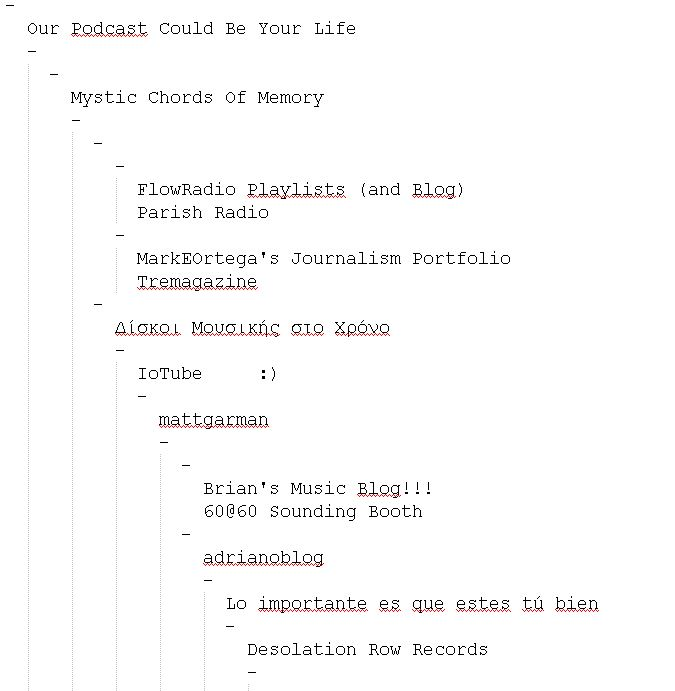
\includegraphics[scale=0.55, keepaspectratio=true]{figures/2.JPG}
\caption{Sample ascii output}
\label{fig:q2fig1}
\end{center}
\end{figure}
\item Furthermore to get the JPEG dendogram I used `clusters.py' and the code from `presentation slide 13'. This code is in Listing \ref{lst:q2code2} 
\newpage
\item The output JPEG that clusters the most similar blogs is illustrated in the Figure \ref{fig:q2fig2}
\begin{figure}[h!]
\begin{center}
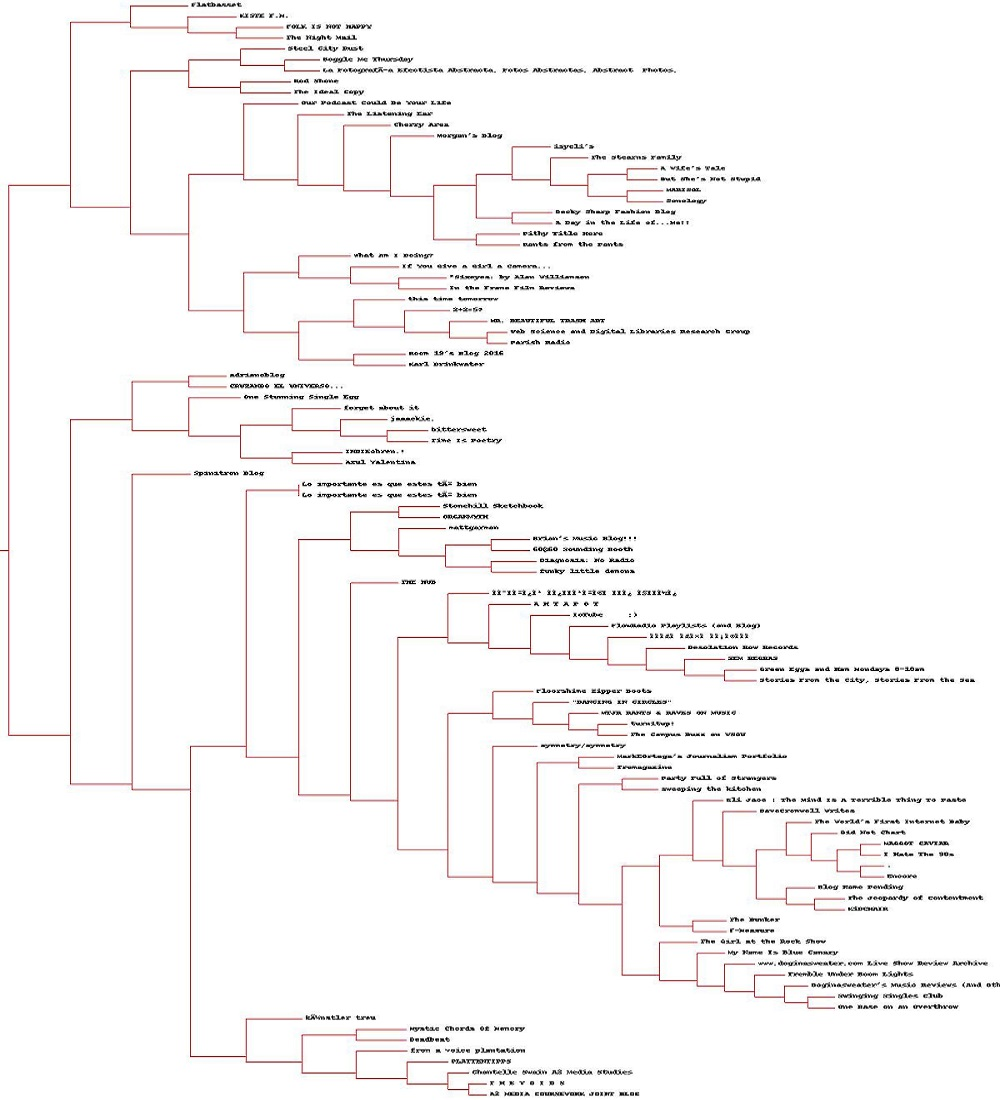
\includegraphics[scale=0.55, keepaspectratio=true]{figures/blogclust.jpg}
\caption{JPEG dendogram}
\label{fig:q2fig2}
\end{center}
\end{figure}
\end{itemize}


\newpage
\textbf{Code Listing}
\sloppy
\lstinputlisting[language=Python,caption=Python code for generating ASCII,frame=single,breaklines=true,label=lst:q2code1, tabsize=2, captionpos=b,numbers=left,showspaces=false,showstringspaces=false,basicstyle=\footnotesize]{src/generateAscii.py}


\textbf{Code Listing}
\sloppy
\lstinputlisting[language=Python,caption=Python code for generating JPEG dendogram,frame=single,breaklines=true,label=lst:q2code2, tabsize=2, captionpos=b,numbers=left,showspaces=false,showstringspaces=false,basicstyle=\footnotesize]{src/generateJPEGdendogram.py}